\documentclass{standalone}
\usepackage{tikz}
\usetikzlibrary{positioning}
\begin{document}
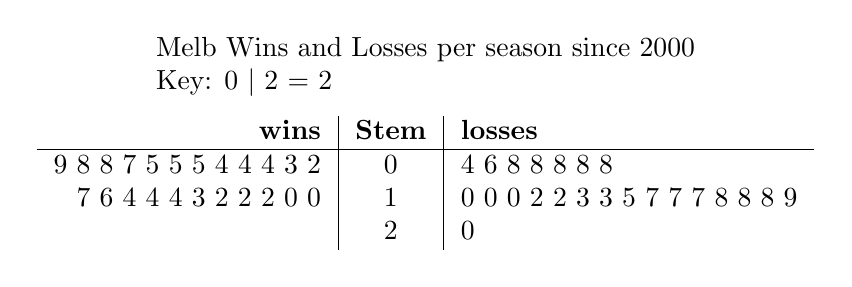
\begin{tikzpicture}
\node[align=left] (top_node) at (0,0) {Melb Wins and Losses per season since 2000 \\ Key: 0 $\vert$ 2 = 2};
\node[below=of top_node,yshift=10mm] {
\begin{tabular}{r|c|l}
\textbf{wins} & \textbf{Stem} & \textbf{losses}\\
\hline
9 8 8 7 5 5 5 4 4 4 3 2 & 0 & 4 6 8 8 8 8 8 \\7 6 4 4 4 3 2 2 2 0 0 & 1 & 0 0 0 2 2 3 3 5 7 7 7 8 8 8 9 \\ & 2 & 0 \\
\end{tabular}};
\end{tikzpicture}
\end{document}